\section{Further Research Trends}

This section is not intended to describe every aspect to its fullest, but to illustrate a showcase of possible and/or desirable developments of VR and HMD in the very near future. \newline
Some mentioned technologies are only predictions and time will show which of these can become a reality in the next couple of years. \newline
Since the leading edge of virtual reality will be computer generated VR for a long time to come these predictions will refer mostly to this~\cite{online:oculusKeynote}. The innovations will find its way into mobile and console VR over time, but the power, compute and pricing advantages will mean that computer generated virtual environments will provide the most complex and convincing experience for a very long time.

\subsection{Improvements For VR Games}
%\subsubsection{General Interaction}
%
%Right now there are the following options available to receive input from a user in the virtual environment.
%\begin{itemize}
%	\item Physical controller
%	\item Voice/sound recognition
%	\item Body tracking
%	\begin{itemize}
%		\item Camera
%		\item Infrared
%		\item Ultrasound
%	\end{itemize}
%\end{itemize}
%
%\todo{describe}
%
%In future applications researchers have to find new interaction methods to receive input of the user. In many VR related companies this research is already starting or fully at it. 
%
%Here are some examples for new interaction methods:
%
%\begin{description}
%	\item[SteamVR controller] New prototypes have a much smaller 'handprint' than what's in the hands of HTC Vive users today. The prototypes are not so much held as they are (optionally) gripped; a band hooking over the side of the user’s palm connects the core of the controller to a sort of backhand gripper which appears to keep the controller attached to the hand even while it isn’t being held.
%	\item[Noitom Hi5 VR Glove~\textcopyright] The first wireless consumer glove designed for virtual reality headsets. You can now have both hands in the game thanks to our IMU sensor technology. 
%\end{description}

\subsubsection{Locomotion}
\label{sec:locomotion}

\begin{figure}
	\centering
	\begin{subfigure}[b]{0.38\columnwidth}
		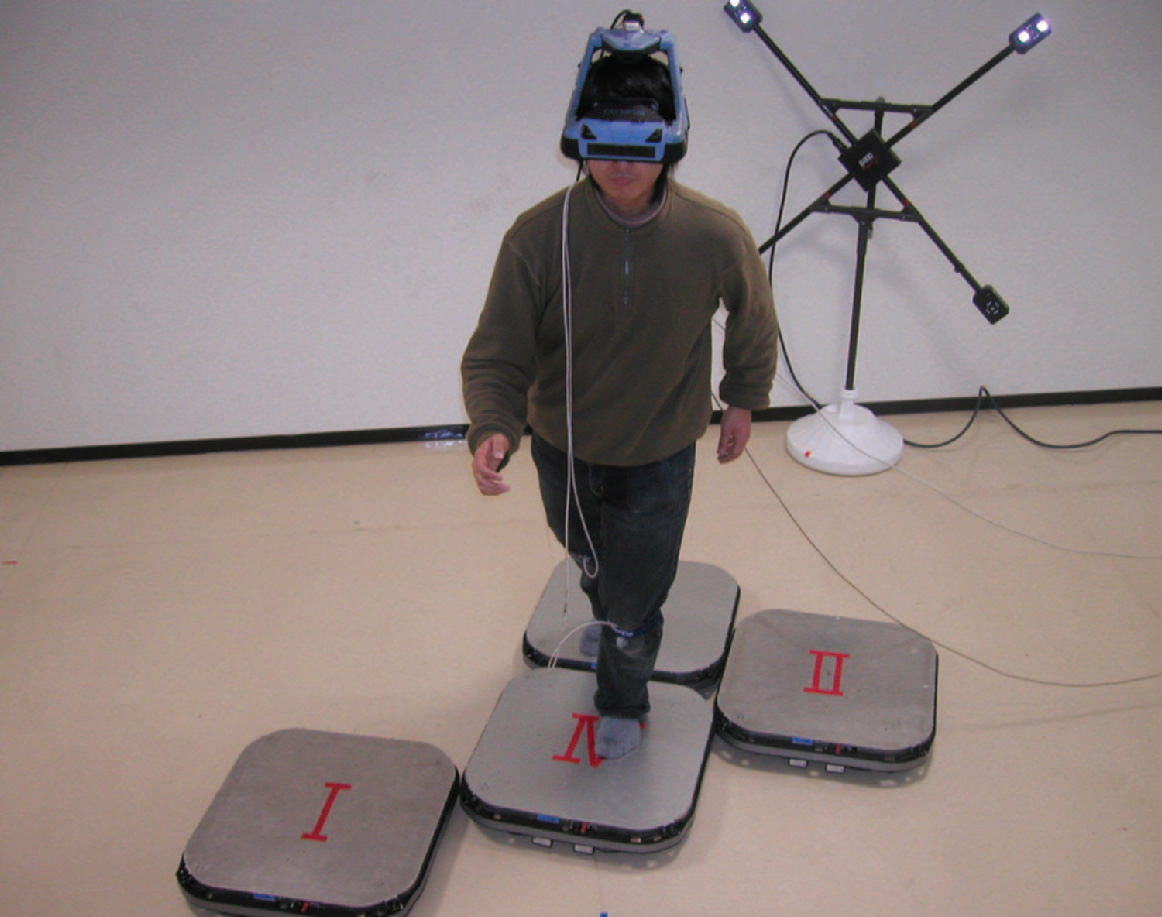
\includegraphics[width=\textwidth]{./figures/01381227}
		\caption{CirculaFloor\newline}~\label{fig:cirFloor}
	\end{subfigure}
	\begin{subfigure}[b]{0.38\columnwidth}
		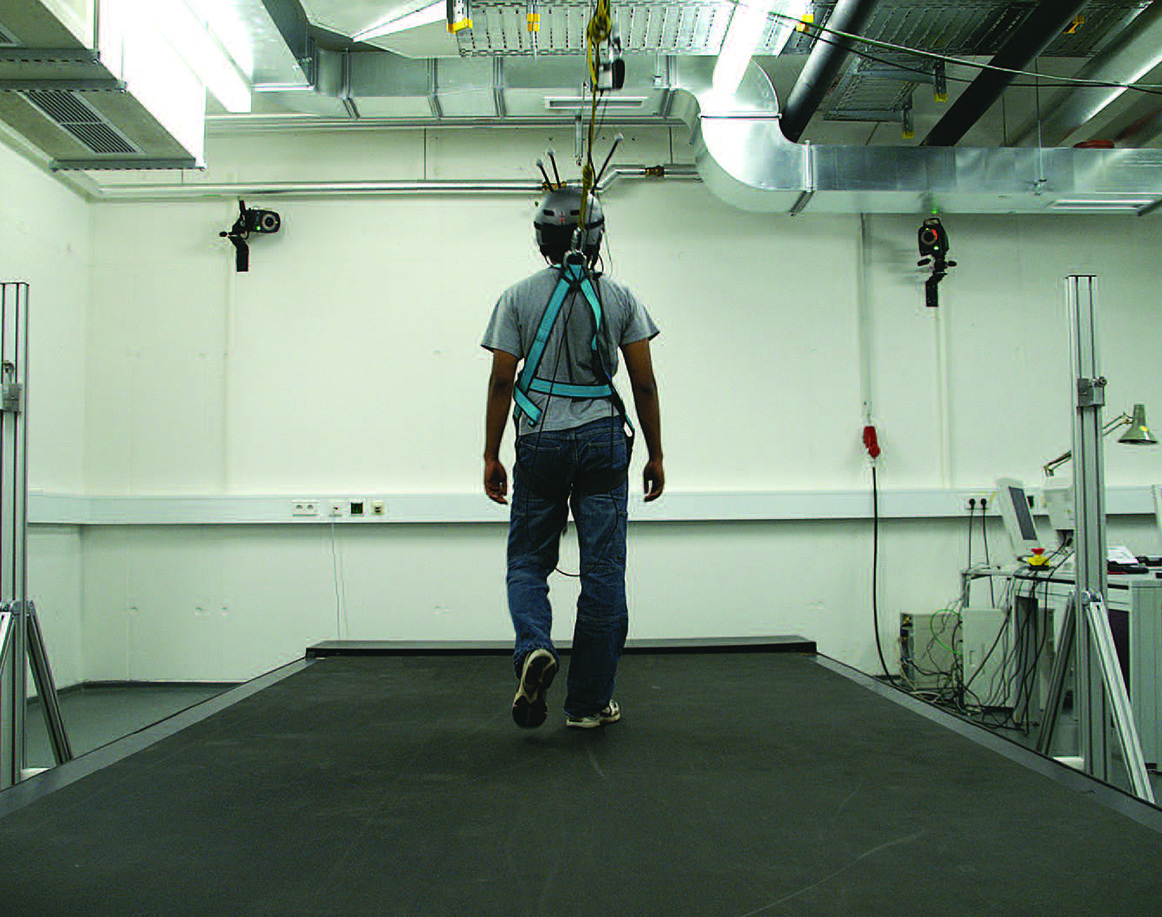
\includegraphics[width=\textwidth]{./figures/ACM_TAP_2010}
		\caption{Omnidirectional treadmills}~\label{fig:omniTread}
	\end{subfigure}
	\begin{subfigure}[b]{0.21\columnwidth}
		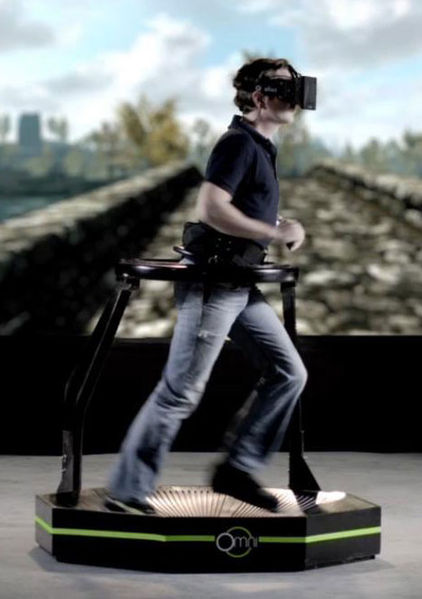
\includegraphics[width=\textwidth]{./figures/422px-Virtuix_Omni_Skyrim_(cropped)}
		\caption{Omni Gaming Treadmill}~\label{fig:virtuixOmni}
	\end{subfigure}
%	\begin{subfigure}[b]{0.89\columnwidth}
%		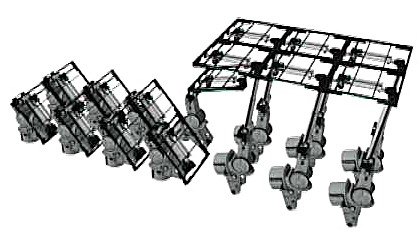
\includegraphics[width=\textwidth]{./figures/portallabrattest}
%		\caption[Portal 2 : Lab Rat Panel Test]{Screenshot from the promotional video 'Portal 2 : Lab Rat Panel Test' (\ccbyncsa) of the game \textit{Portal 2 \textregistered\textcopyright} showing the general setup of floor panels mounted to robotic arms. This method enables developers to modify the structure of the floor at runtime.\footnotemark}~\label{fig:portallabrattest}
%	\end{subfigure}
	\caption[]{Left: The CirculaFloor using movable floor tiles to simulate a larger traversable area. | Middle: The omnidirectional treadmill used for the development of the algorithm used by Souman et. al. | Right: The Omni Gaming Treadmil from Virtuix developed to simulate large play areas for gaming. Image source in footnote 4\textcolor{white}{\footnotemark[4]}}
\end{figure}

\footnotetext[4]{~Figure~\ref{fig:cirFloor}: CirculaFloor~\cite{Iwata:2005:CLI:1078037.1079777}, Iwata et. al. | Figure~\ref{fig:omniTread}: Making Virtual Walking Real~\cite{Souman:2010:MVW:1670671.1670675}, Souman et. al. | Figure~\ref{fig:virtuixOmni}: Omni Gaming Treadmill \url{https://upload.wikimedia.org/wikipedia/commons/f/fd/Virtuix_Omni_Skyrim_(cropped).jpg}~\ccbysa}

Existing locomotion techniques have huge advantages but also disadvantages regarding immersion, simplicity and health aspects. It is a very comprehensive field of studies and research to optimize the illusion provided by a virtual environment by using better approaches towards the transition of the in game character.\newline
To enable the player to move freely inside the virtual environment different devices and techniques have been developed to offer artificial locomotion to the user. The main goal is to create a space where the user can move freely in all 3 axes at best and therefore gain an ideal gaming experience.\newline
The following approaches have been made by researchers to enable the player to move around in the in game world without the need of a large area designed like the game itself. These will be categorized under \textit{artificial locomotion} where the device described display another interface for the user to interact with, but will bypass the problems of this interaction method since the users senses receive a more persuasive feeling of movement.
\begin{description}
%	\item[Point \& teleport locomotion] In this technique, users simply point where they want to be in virtual world and they are teleported to that position. As a major advantage, it is not expected to introduce motion sickness since it does not involve any visible translational motion. Advantages and possible alternatives are described in \textit{Point \& Teleport Locomotion Technique for Virtual Reality}~\cite{Bozgeyikli:2016:PTL:2967934.2968105}
	\item[CirculaFloor] Approaches like the one taken by Hiroo Iwata, Hiroaki Yano, Hiroyuki Fukushima in their CirculaFloor~\cite{Iwata:2005:CLI:1078037.1079777} as seen in Figure~\ref{fig:cirFloor} have shown that shape changing interfaces are generally not hard to build. It was aimed to design a new hardware architecture that would be easy to upgrade the actuation mechanism or add new mechanisms for the creation of uneven surfaces. To achieve these goals, a configuration for a locomotion interface using a set of omnidirectional	movable tiles was designed~\cite{Iwata:2005:CLI:1078037.1079777}. \newline Each tile is equipped with a holonomic mechanism that achieves omnidirectional motion. An infinite surface is simulated by the circulation of the movable tiles. Position sensors measure the motion of the feet. The tile moves in the opposite direction of the walker’s measured direction, canceling the motion of the step~\cite{Iwata:2005:CLI:1078037.1079777}. This computer-controlled motion of the tiles fixes the walker’s position. The circulation of the tiles can cancel the walker’s displacement in an arbitrary direction. Thus, the walker can freely change direction while walking~\cite{Iwata:2005:CLI:1078037.1079777}. 
	
	\item[Omnidirectional Treadmill Algorithm]Another approach made by Souman et. al.~\cite{Souman:2010:MVW:1670671.1670675} shows the potential for omnidirectional treadmills. They developed an algorithm to steer the speed of a treadmill in such a way that VR immersiveness is not disrupted by changes in treadmill velocity. "This algorithm was developed to work with an omnidirectional treadmill ...", as shown in Figure~\ref{fig:omniTread}, "... allowing for changes in both walking speed and direction"~\cite{Souman:2010:MVW:1670671.1670675}. "A user can therefore walk in place and the VR system defines the world around him as endless space".~\cite{Souman:2010:MVW:1670671.1670675}\newline This approach tackles problems better than the CirculaFloor because it generates less disturbance in the users walking pace.
	
	\item[Omni Gaming Treadmill] Is an omnidirectional treadmill being developed by \textit{Virtuix}. Their \textit{Omni Gaming Treadmill~\textcopyright} can be seen in Figure~\ref{fig:virtuixOmni}. The Omni uses a concave, low-friction platform that enables a smooth gait and immersive walking and running motion.~\cite{online:omni}
	
%	\item[Portal]A third approach has been made by the game developers of the game PORTAL. Building rooms completely out of tiles controlled by robotic arms can outline a whole room. Configurable, expendable and in moderate size. Combining this with VR holds great potential to create the perfect illusion. A schematic portrayal of this functionality can be seen in Figure~\ref{fig:portallabrattest}
%	An imaginable application is when the tiles are intelligently configured to 'disappear' (into the ground) behind the player and appear in front of him kind of like a hamster wheel, making the playable area seem infinitely large to the player. The principle would be similar to the one described in CirculaFloor where the main disadvantage is that the floor tiles are unstable and not yet matured enough to provide sufficient support when walking at normal speed.
\end{description}

Usable research to \textit{cockpit} and \textit{natural locomotion} have not yet sufficiently been made or could not been found in a satisfactory manner. The approaches towards these locomotion techniques remain a broad field of study for further research. 

In todays VR games 'virtual walls' are a widely seen solution to prevent people from walking into physical items like furniture, walls, stairs et cetera. It is interesting to notice that this is important because VR is not yet ready to support full shape recognition of objects in the living room. With this the HMD could detect hazardous situations or items and the game could substitute it as something the user might not want to touch. The experience provided by this would be more seamless.\newline
Shape recognition could also be important to develop to actively steer the users attention into directions that are open and save for the user to walk towards. On the downside the base station of the VR system must have an enormous amount of computational power to make these kind of calculations.

Useful approaches could be the research known as 'redirected walking', where the user perceives a straight line of walking in game where he is walking in a curved line in real life~\cite{razzaque2001redirected}. The game conveys the impression of a linear forward motion and utilizes a limited amount of space in this manner.

%\begin{figure}
%	\centering
%	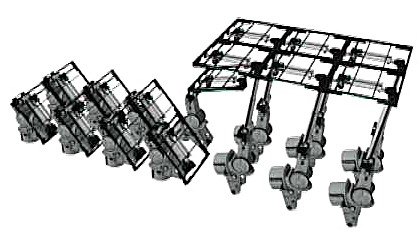
\includegraphics[width=0.89\columnwidth]{./figures/portallabrattest}
%	\caption[Portal 2 : Lab Rat Panel Test]{Screenshot from the promotional video 'Portal 2 : Lab Rat Panel Test' (\ccbyncsa) of the game \textit{Portal 2 \textregistered\textcopyright} showing the general setup of floor panels mounted to robotic arms. This method enables developers to modify the structure of the floor at runtime.\footnotemark}~\label{fig:portallabrattest}
%\end{figure}
%\footnotetext{\textcopyright~Valve Software, Portal 2, [Online; accessed November 05., 2016],[Digitally revised] \url{https://www.youtube.com/watch?v=S7vFxs0ycn0}}

\subsubsection{Sight}

Head mounted displays of today have far less pixel density, a narrower field of view (FOV) and the lenses used have no actual method of actively focusing what the user is looking at~\cite{online:oculusKeynote}.\newline
It is important to understand that a result of human evolution is that the visual perception ot things affects the impression we get of something in an enormous way. \newline
To improve the visual representation and the image transmitted by HMDs the work on pixel density together with field of view will be standing in focus on future research iterations. It has mainly two approaches which accompanies an interesting trade-off in the usage of the resulting display resolution. Pixel density is a function of both, display resolution and field of view. One can have a higher pixel density image with a narrower field of view, or a wider field of view with a lower pixel density image~\cite{online:oculusKeynote}. \newline
It all depends on what FOV is achievable and how compelling a wider FOV turns out to be.

The two approaches are to either achieve a generally higher pixel density and with that a higher resolution on the displays or to teach the system to recognize the field of focus of the user.

A wider field of view with higher resolution will require a breakthrough in optics. Todays available lenses have a limited field of view without noticeable distortion, so new optics technology will be required~\cite{online:oculusKeynote}. This is not limited to newer or more advanced lenses but also so self adapting settings regarding distance, orientation and yaw of these. 

The used lenses of HMDs have also a fixed focus and while the human eye can adapt to different distances between objects the lenses of today stay focused around a distance of two meters~\cite{online:oculusKeynote}. This would require an entirely new lens technology synthesizing on technologies like varifocal glasses, but adapting to the position the user is looking at.

The last point can be addressed with research field like \textit{holographic displays}, \textit{light field displays}, \textit{multifocal displays} or \textit{varifocal displays} and todays research teams are already on the subject~\cite{online:oculusKeynote}.

\subsubsection{Touch}

Touching something in VR and receiving real feedback from an in game object can expand the illusion of a real virtual environment. \newline
Using some similar technology to the iDummy~\cite{online:idummy} developed by Chan et. al. developers can create various objects of different size and shape. A user wearing a VR Headset could see a specific object and feel it as if it was the real thing. Using the technology developers can extend the realm of VR to one more dimension. Together with the technology of Mahdi Azmandian et. al. in their paper \textit{Haptic Retargeting: Dynamic Repurposing of	Passive Haptics for Enhanced Virtual Reality Experiences}~\cite{Azmandian:2016:HRD:2858036.2858226} the technology could be even further expanded to having a multitude ob objects of different shapes, size and orientation in ones direct vicinity. This could enable developers to enter unknown territory of unforeseen possibilities. 

The iDummy is a mannequin technology where different body parts can be modified by using multiple servo motors. The mannequin can change its chest circumference as well as hip measurement or the width of the waist to adapt to the needs of apparel designers and represent every body shape imaginable. \newline
Haptic retargeting is the process of making the user think he is touching different objects by differentiation between them in virtual space~\cite{Azmandian:2016:HRD:2858036.2858226}. In reality these objects might be the same. 

Adapting these principles to basic shapes, like cubes, balls or tetrahedrons a very haptic way of interacting with in game objects can be pursued. A user wearing a HMD can actually touch an object, feel its presence and the device is adding a visual abstraction casuing the user to belive what he is touching is real. The player could with this method touch a ball of moderate size and see a basketball in the virtual representation of this.

Comparable research has been done on shape changing interfaces, in example by Rasmussen et. al.~\cite{Rasmussen:2012:SIR:2207676.2207781}. They define 8 types of change for objects in 2 categories:

\begin{description}
	\item[Topologically equivalent] Change of \textit{orientation}, \textit{form},  \textit{volume}, \textit{texture} \textit{viscosity} and \textit{spatiality}.
	\item[Not topologically equivalent] \textit{Addition or subtraction} and \textit{permeability} of materials.
\end{description}

With modifications to the object a person is holding often comes the impression of irreality if just minor features of this objects are not as expected by the person interacting, i.e. if the surface of one object feels smooth but the virtual representation of the object shows a rough stone the user knows something is off. \newline
Psychologically the subject needs to be investigated since no proposition regarding divergent perception using HMD have been made.
%
%Further Azmandian et. al. have already approached the topic of dynamic retargeting in their publication \textit{Haptic Retargeting: Dynamic Repurposing of Passive Haptics for Enhanced Virtual Reality Experiences}~\cite{Azmandian:2016:HRD:2858036.2858226}. The goal was to create a design space where game developers may reuse the physical objects in a person’s vicinity to provide a sense of touch when reaching, grabbing, lifting, or otherwise manipulating artifacts in a virtual reality scene, but to not be limited by what specific objects are around and whether they are located in the ''right'' place.

\subsubsection{Smell}

There are almost no studies what smell provides for virtual reality and this subject is hard do depict and predict. Over all smell provides yet another dimension of immersion to a virtual environment and is after all one of the five basic senses of man, although negligible compared to visual, acoustic and haptic perceptions.

\subsubsection{Taste}

Similar to the sense of smell taste is a dimension of interaction not seen by many games. Virtual reality at this moment offers no way of tasting something seen in a virtual environment. This has also not been addressed in other applications, but research has been made. There are times when a user might want to percept a taste and other times when we would hope not to do so, same goes for the smelling aspect of games et cetera.

Ranasinghe, Nimesha and Do, Ellen Yi-Luen~\cite{Ranasinghe:2016:VSS:2984751.2985729} have developed a way to address the taste buds using electrical stimulation. The proposed method is built on existing research that has highlighted the possibility of generating taste sensations by heating and cooling the human tongue. Right now they have only simulated sweet sensations, as described in \textit{Virtual Sweet: Simulating Sweet Sensation Using Thermal	Stimulation on the Tip of the Tongue}, but said other tastes would also be imaginable~\cite{Ranasinghe:2016:VSS:2984751.2985729}.

Unresolved remains the question of how this be included in the HMD. It would be impractical to attach a mask to the devices just to have taste and smell in a game. HMDs are already bulky and sometimes impractical so for most applications adding another device to the headset would disturb more than it would help.

\subsubsection{Hearing}

Humans can locate sounds in three dimensions – in approximate distance and direction. This is possible because the brain, inner ear and the external ears work together to make inferences about location.\newline
An Head-Related Transfer Function (HRTF) describe how audio has to be produced with a limited amount of audio sources to give the illusion that a sound is coming from a given point in space.\newline
How sound reflects, diffracts and interferes with objects in VR is an important point for the future, so sound propagation has to be researched further as VR games get developed~\cite{online:oculusKeynote}. Alongside with HRTFs the illusion in the virtual environment can be further enhanced.

Continuing, researchers of the next decade have to tackle the problem of attention steering. Sound can be very helpful in getting a user to turn his head in one direction or to prevent him from bumping into objects located in the area he is playing a VR game. This can be helpful along with virtual walls, as described in the section \textit{Locomotion~\ref{sec:locomotion}} from above.

But sound can also be used to interact with VR devices. For a convenient method of interaction with VR systems that do not usually use controllers, such as the \textit{Samsung Gear VR} or \textit{Daydream View}, Zayer, et. al. have developed the PAWdio~\cite{Zayer:2016:PHI:2967934.2968079}, a method to determine the general position of the users hand using acoustic sensing. It works by emitting sound waves in ultrasound spectrum, from earphones that the user is holding in his hands, that can be ascertained by the mobile headset to calculate the users hand position and orientation. The method uses physical circumstances like the Doppler effect to calculate the users hand position~\cite{Zayer:2016:PHI:2967934.2968079}. Compared with vision based sensing it can be implemented with little computational overhead. \newline
Although some problems are given naturally by this method it provides a basic approach to take VR to every smartphone and with that to many more people than before.

%\subsection{Health Aspects}
%
%\begin{description}
%	\item[Virtual reality sickness] \textit{(Also cybersickness)} Occurs when exposure to a virtual environment causes symptoms that are similar to motion sickness. \newline The most common symptoms are general discomfort, headache, stomach awareness, nausea, vomiting, pallor, sweating, fatigue, drowsiness, disorientation, and apathy. \newline Virtual reality sickness is different from motion sickness in that it can be caused by the visually-induced perception of self-motion; real self-motion is not needed.
%\end{description}
%
%Cybersickness has been discussed by Kay M. Stanney, Robert S. Kennedy and Julie M. Drexler back in 1997~\cite{stanney1997cybersickness}. Studying the symptoms and their effects on test subjects they found that users where experiencing cybersickness on different levels. In order to provide a context, he suggested that individuals who report symptoms which tally higher than 15 on the Simulator Sickness Questionnaire, would be experiencing sufficient discomfort that, unless there were other incentives, they would not voluntarily seek additional exposure because of the level of discomfort. 
%
%It is found that cybersickness is a problem that must be corrected in order for virtual environments to be usable by anyone who wishes to use them~\cite{lo2001cybersickness}. So the important question arises as to how one can eliminate cybersickness or at least reduce its severity so people who are susceptible to cybersickness can use virtual environments.
%
%It is a subject of investigation how health games can be beneficial for users. Virtual reality might not be the best purpose for games intended to increase the physical health of users, but until now no company has tackled the subject with medical support or professional health training advice. Other devices like the Wii fit with the balance board have shown that the demand for entertaining training is existent.
%Using this HMD need to be a lot lighter than they are today. Also they have to be developed to be more ergonomic and comfortable to wear.
%
%VR games could be used to help in the treatment of people with mental problems. Since VR is more immerse than 'normal' games it could be discovered that people suffering from asperger syndrome benefit from games in VR and head mounted devices.
%Also VR game developers must research what is with people who suffer from anxiety disorders. It it important to know the downside of virtual environments and the immerse way that can sometimes evoke anxiety states from frightening situations experienced in games. A suggestion is that games offer different degrees of abstraction or alienation to differentiate between VR and the real world. The user can thereby choose the level of immersion himself.

\subsection{Increasing The Performance Of Devices For VR Gaming}

The performance of VR systems especially of mobile and console systems has to be increased to convey a sophisticated illusion of mobile VR. In most parts this will not be required for the majority of applications but if the industry is able to establish new markets the development of VR might even proceed faster.

The performance of the base station is mostly stable when users have high performance systems at home, but when the system is not capable of delivering the required computational power the frame rate can vary a lot. \newline
A frame rate that is too low might be one of the biggest causes of virtual reality sickness. \newline
With \textbf{virtual reality sickness} a user can experience symptoms very similar to motion sickness. This will include discomfort, headache, stomach awareness, nausea, drowsiness, disorientation, apathy and other symptoms similar to sea sickness. Virtual reality sickness is different from motion sickness, because it can be caused by a moving image, rather than actual motion itself. Virtual reality sickness can be best categorized in disorientation. This 

The issue laying behind this is caused to the refresh rate of the screen. When the frame rate is changing or not matching evenly with the refresh rate of 90Hz for modern HMDs, the user gets perceived judder or tearing and other phenomenons. For VR it is generally quite uncomfortable if the system cannot deliver the needed power.

This will in most parts be handled over time when the performance of other systems reaches the performance of computers. Most parts of mobile systems, i.e. smartphones have developed computational strength of computers from a few years ago. Moore's law is applying to any digital system.

Regarding wireless connections to the base station the first approaches towards a more mobile experience have been made by HTC Corporation with the new technology named \textit{''VIVE tether-less upgrade kit''}~\cite{online:tpCast} developed by TPCAST. \newline
In November 2016 HTC has unveiled a tether-less VR upgrade kit for VIVE VR systems. It was developed and produced by TPCAST. This kit will enable users of high-end PC VR systems to have a fully untethered experience without compromising quality~\cite{online:tpCast}. It is archived by using advanced mobile connections from the base station to the headset.\newline
Advantages of this are the gained space opportunity and mobility within the gaming area.
